% proposal.tex
\documentclass[12pt]{article}
% preamble.tex

% enclose any latex in \comment{} to suppress it
\newcommand{\comment}[1]{}
\newcommand{\citeNP}[1]{\cite{#1}}

\usepackage{graphicx}
\usepackage{subfig}
\usepackage{multicol}
\usepackage{times}
%\usepackage{floatflt}
\graphicspath{{./}{figures/}}

% NO psfig -- pdflatex does not support it ...
% \usepackage{psfig}
% \psfigurepath{./:figures/}
% \DeclareGraphicsRule{.eps.gz}{eps}{.eps.bb}{'gunzip -c #1}

\newcommand{\upline}{\vspace*{-\baselineskip}}
\newcommand{\up}{\vspace*{-6pt}}
\newcommand{\downline}{\vspace*{\baselineskip}}
\newcommand{\sep}{~~~~~~~~~~}

% this hardcodes the bib name, which we don't want to do.
% \renewcommand{\thebibliography}[1]{\section*{References Cited}
% \addcontentsline{toc}{section}{References Cited}\list
%  {[\arabic{enumi}]}{\settowidth\labelwidth{[#1]}\leftmargin\labelwidth
%  \advance\leftmargin\labelsep
%  \usecounter{enumi}}
%  \def\newblock{\hskip .11em plus .33em minus -.07em}
%  \sloppy\clubpenalty4000\widowpenalty4000
%  \sfcode`\.=1000\relax}

% fix this to specify width and height, and solve for the margins
% margins.tex

% import calc
\usepackage{calc}

%
\newlength{\myrightmargin}
\newlength{\myleftmargin}
\newlength{\mytopmargin}
\newlength{\mybottommargin}

% Change these settings to change the margins
\setlength{\myrightmargin}{1.0in}
\setlength{\myleftmargin}{1.0in}
\setlength{\mytopmargin}{0.75in}     
\setlength{\mybottommargin}{0.75in} 
\setlength{\oddsidemargin}{0.0in}   % extra room on inside side

%%% use margin settings to set width variables
\setlength{\evensidemargin}{0 in}
\setlength{\marginparsep}{0 in}
\setlength{\marginparwidth}{0 in}
\setlength{\hoffset}{\myleftmargin - 1.0in}
\setlength{\textwidth}
  {8.5in -\myleftmargin -\myrightmargin -\oddsidemargin}

%%% use margin settings to set height variables
\setlength{\voffset}{\mytopmargin -1.0in}
\setlength{\topmargin}{0 in}
\setlength{\headheight}{12 pt}
\setlength{\headsep}{20 pt}
\setlength{\footskip}{36 pt}
\setlength{\textheight}
  {11.0in-\mytopmargin-\mybottommargin-\headheight-\headsep-\footskip}

% \oddsidemargin 0.2cm
% \evensidemargin 0cm
% \textwidth 16.0cm
% \topmargin -1.25cm
% \textheight 22.94cm

% remove parindent, squeeze grafs
\setlength{\parindent}{0in}
\setlength{\parskip}{1ex}

\def\nibf#1{\noindent\textbf{#1}}


\date{\today}

\author{
David J. Lilja\\
University of Minnesota\\
200 Union St. SE \\
4-174 Keller Hall \\
Minneapolis, MN 55455}

\title{Resource Management using Statistical Inference\\
in Virtualized Environments}

\begin{document}

\bibliographystyle{plain}
\setcounter{page}{1}

\maketitle


\newpage

\pagestyle{plain}
\setcounter{page}{1}

\section*{Abstract}

Blah blah blah blah

\section{Introduction}
\label{introduction}

The primary objective of this project is to automatically map a given application�s requirements to physical hardware resources such that the application performance can be maintained in a highly consolidated virtual machine environment. In our previous work with VMware, we developed a storage performance modeling framework called Romano. 
This new model differs from the previous model, Pesto \cite{pesto}, which is currently in use in the \emph{Virtual Center} product, in that it identifies the key characteristics of a workload that affects the performance using statistical analysis of variance (ANOVA) \cite{lilja}.
The resulting prediction accuracy is improved by about 80\% allowing much more aggressive load balancing when using Romano than with Pesto. As a comparison, the residuals from both techniques are shown in Figure \ref{residualDist} for four different storage systems.

While this approach is very good at predicting the performance of a data store, it currently lacks the ability to predict the performance for each virtual disk when they are consolidated onto a single data store. The main focus of this project will be to extend the Romano approach to predict the performance of each virtual disk when they are consolidated onto single data stores.

\begin{figure}[ht]
\centering
\subfloat[Pesto]{\label{rdPesto}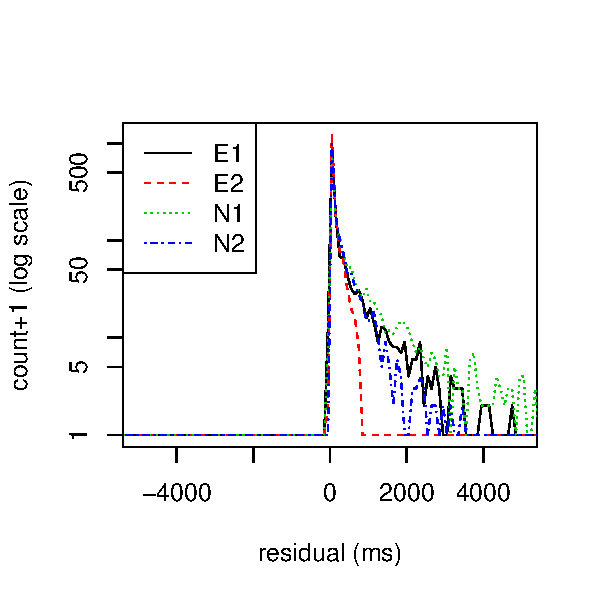
\includegraphics[width=0.4\columnwidth, clip, trim=0 0.5in 0.2in 0.3in]{error_hist_compare_pesto.pdf}}
\subfloat[Romano]{\label{rdRomano}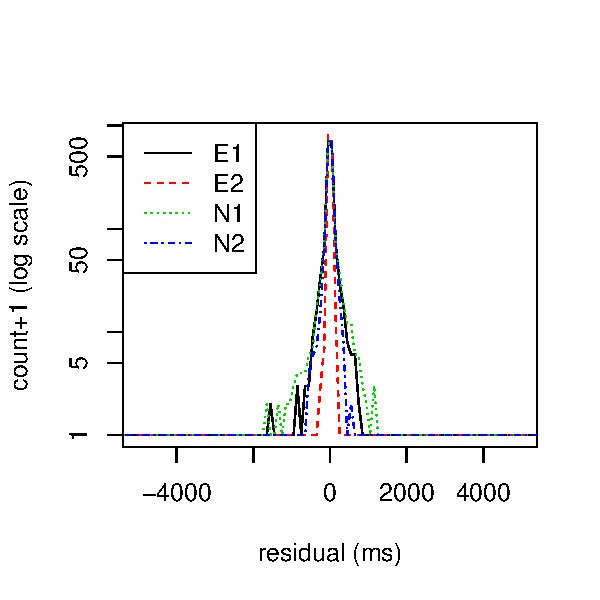
\includegraphics[width=0.4\columnwidth, clip, trim=0 0.5in 0.2in 0.3in]{error_hist_compare_kromano.pdf}}
\caption{Distribution of residuals ($\epsilon$) for Pesto and Romano.
The x-axis is the value of $\epsilon$ in $ms$.
The y-axis is number of occurrences+1.
(The addition of 1 was required to allow the y-axis to be plotted in a log scale.)
%The $\epsilon$ distribution does not change widely for Romano indicating that the accuracy of Romano is less dependent on the data store than the Pesto model. 
Furthermore, Romano's $\epsilon$ values are symmetric around 0, indicating that its residuals are unbiased.
}
\label{residualDist}
\end{figure}

\section{Limitations of Prior Work}

The results of our Romano\cite{romano} project reveal that the workload and storage models are highly interdependent for certain class of workloads. 
This result confirms observations from other prior work~\cite{relative-fitness, benchmark}.  
%Whereas techniques based on independent models have been shown to have good average-case behavior, they work suffers from severe corner case model inaccuracies. 
%These can lead to expensive bad data movement recommendations. 
%Furthermore, the cost-benefit analysis in earlier work has largely ignored the time-series nature of the workload interference into account, further eroding accuracy.
Early efforts to automatically manage storage resources in a virtualized environment, such as \emph{VectorDot}~\cite{vectordot}, ignored the workload and simply concentrated on the utilization of each storage system. 
A workload from the over-utilized device was simply migrated over to a less utilized device. 
This approach fails to work in a heterogeneous storage environment since the resulting performance on each different type of data store is unknown.
Furthermore, the goal is not to ensure that no storage system suffers from over-utilization but rather to ensure that no workload suffers from degraded performance. 

Other work has focused on highly accurate latency prediction of workloads across storage devices.  However, these predictors have come at the expense of practicality by requiring extensive off-line experimentation and modeling. 
For instance, Wang et al~\cite{relative-fitness} developed the CART models off-line to develop workload-storage models. 
In contrast to their work, our proposal is to learn storage behavior quickly using online statistical calibration without resorting to expensive and cumbersome off-line methods.

\section{Proposed Architecture}
\label{sec:technical}

Our proposed prediction and management architecture is shown in Figure~\ref{arch}.
The virtualization layer will provide the framework to partition the available hardware resources and to isolate the performance interference between them \cite{vmware5}. 
The management layer will provide the means to create a \emph{pool} of resources from a cluster of heterogeneous machines \cite{drs}, which will increase the total amount of resources available for mapping. 
Live migration techniques \cite{nelson2005fast,clark2005live,mashtizadeh2011design} allow applications to be remapped based on the time-varying demands of the applications and the availability of the physical machines. 
These mechanisms already exist in the current virtualization infrastructure.
However, the mapping itself is still carried out manually, which decreases the benefits of virtualization and exposes the system to human error. 

\begin{figure}[ht]
\centering
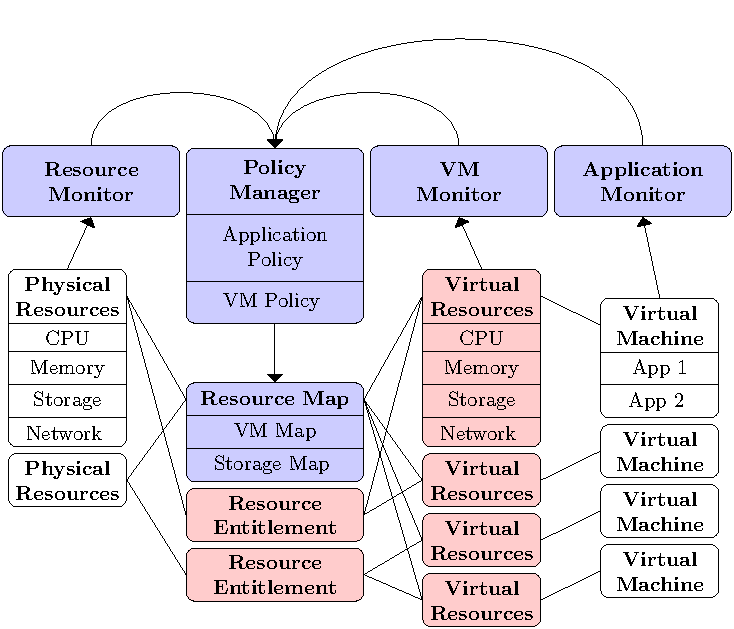
\includegraphics[width=0.9\columnwidth, clip, trim=0 0in 0 0.2in]{archfig.pdf}
\caption{Overview of the proposed architecture. The blue modules are implemented in the \emph{Virtual Center} server and have a global view of the entire system. The red modules are implemented in the \emph{ESXi} server and have the local host view.}
\label{arch}
\end{figure}

To achieve our objective, the system must be aware of the workload changes and be able to remap the resources to ensure that remapping satisfies the requirements of all active applications.
Significant progress has already been made to migrate virtual machines to load balance CPU and memory resources \cite{nelson2005fast, clark2005live}.
However, correct I/O performance prediction is a much harder problem due to the available state information in storage systems \cite{basil}.
Another problem is that virtualization fails to isolate the performance interference of consolidated I/O workloads as well as it isolates the CPU, memory, and network resources. 
Finally, the last problem is the lack of mapping between the application requirements and the virtualized resources since
the actual application requirements are typically not specified in terms of resource usage. 
Instead they are typically determined by the end user demand that needs to be satisfied.
Our approach addresses these issues using the resource management mechanism and the resource management policy described in the following sections.

\subsection{Resource Management Mechanism}

There are three ways to allocate resources to a VM. 
The simplest approach is through VM configuration. 
However, this approach typically requires a reboot of the VMs and is not the focus of this proposal. 

The second approach is through \emph{entitlement} control, which
is shown as \emph{Resource Entitlement} in Figure \ref{arch}.
The term entitlement refers to the resource scheduling priority in the case where multiple VMs compete for the same resource \cite{parda}.
By giving a higher entitlement of resources to a VM, the effect of consolidation can be minimized.
This approach is especially effective in the case of over-provisioning.
The limitation of this method is that the VM is confined to the physical resources of the current host. 

The third approach to allocate resources is through \emph{live migration}, shown as \emph{Resource Map} in Figure \ref{arch}.
By dynamically relocating VMs onto a more available and powerful system, a VM can potentially access any physical resource available in the system. 
Note that the storage resources are typically a separate entity from the host and require a separate migration path. 
Therefore, we assume that all hosts and storage nodes are fully connected. 

These approaches determine how the virtual resources are mapped to the physical resources.  Their relationship is shown in Figure \ref{arch}.

\subsection{Resource Management Policy}

The resource management policy determines how resources should be allocated.  It is enforced by the \emph{Policy Manager}. 
There are two types of policies, VM policies and application policies. 

The VM policy is a mandatory policy that must be specified when a VM is created. 
This policy includes things such as the number of CPUs, the size of the memory and the entitlement of these resources. 

The application policy is an optional policy that provides a particular application a performance guarantee. 
A given application policy has a higher priority than the VM policy and may override the VM policies if necessary. 
If the dynamic resource management mechanisms cannot satisfy the policy, the \emph{Virtual Center} server may issue a warning and recommend that the VM be reconfigured.  This requires reboot of the VM. 

To ensure that the policies are met and will continue to be likely to be met in the future, current system states are continuously monitored. 
A resource monitor checks the health status of the physical resources as well as monitors the addition of new resources. 
The VM monitor checks the health of the VMs as well as their current performance and resource requirements. 
The application monitor collects the application performance statistics.  It requires support from the guest OS. 

Given the policies and monitored information, the policy manager decides how the resource mapping and entitlements should be configured. 
This will be the focus of our work.
To determine what mapping and entitlements will satisfy the policy with minimum resources, we must be able to predict the performance after the changes. 
We propose to use statistical inference techniques to model the VM level performance and/or the application level performance based on the workload and the resources provided. 
The modeling framework will first extract the characteristics from the workload such that these extracted characteristics have high correlation with the performance. 
These characteristics then will be regressed against the performance under various resource configurations to determine the performance model. 

\section{Statement of Work}
\label{plan}

We are proposing a three-phase project. 

The first phase will develop an approach to predict the performance of a virtual disk given a workload and a storage system. This phase will produce a virtual disk performance model. 

The second phase will model the performance interference between different virtual disks on a single storage system. 
We will apply statistical inference to understand the effect of interference to derive each VM's I/O performance without having to actually change the system state.  
This approach will allow system administrators to simulate their configuration changes in large scale data centers without disrupting their operation. 
This additional information will be incorporated into the virtual disk performance model of phase one.

The last phase will use these models to map the application requirements to the available resources.
This will allow users to simply specify the desired behavior without having to worry about product details.

By the end of year 1, we expect to determine pseudo-optimal virtual disk placements such that the performance requirements of each virtual disk are satisfied with a minimum number of storage systems.
By the end of year 2, we expect to meet the various application requirements by dynamically mapping resources and performing necessary migrations. 

\section{Preliminary Budget Estimate}


\renewcommand{\refname}{References Cited}
% generate References Cited section
\bibliography{refsA}


\end{document}

